\subsection{Registrering på PDF}\label{sec:PDF}
Dette afsnit indeholder en gennemgang af den grafiske brugergrænseflade, design og implementering af 'Registrering på PDF' viewet i Rambøll Tilsyn.

\subsubsection{Design}
Herunder ses sekvensdiagrammerne for registrering på PDF. \\
Det første sekvensdiagram, som ses på Figur \ref{fig:LoadPDFSekvensDiagram}, viser hvordan PDF-tegningen bliver loadet ind i applikationen.
\begin{figure}[H] % (alternativt [H])
	\centering
	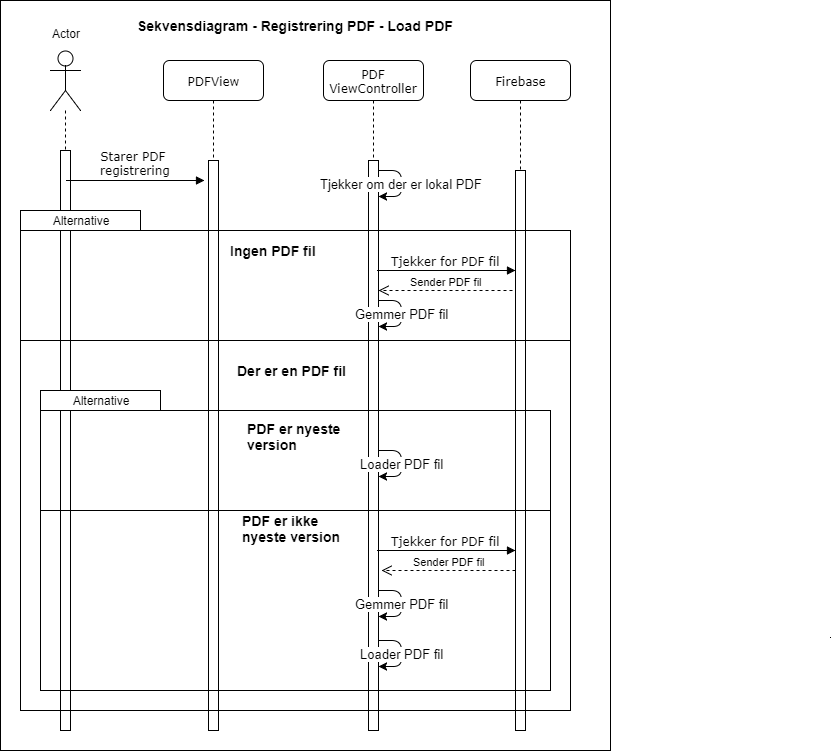
\includegraphics[height=12cm, width=15cm]{../ArkitekturDesign/Design/RegisterPDF/LoadPDFSekvensDiagram}
	\caption{Sekvensdiagram for Registrering på PDF - Loading af PDF, i Rambøll Tilsyn.}
	\label{fig:LoadPDFSekvensDiagram}
\end{figure}

\clearpage

Næste sekvensdiagram, som ses på Figur \ref{fig:LoadJSONSekvensDiagram}, viser hvordan JSON-filen bliver oprettet. Sekvensen med JSON sker direkte efter at PDF sekvensen er overstået.
\begin{figure}[H] % (alternativt [H])
	\centering
	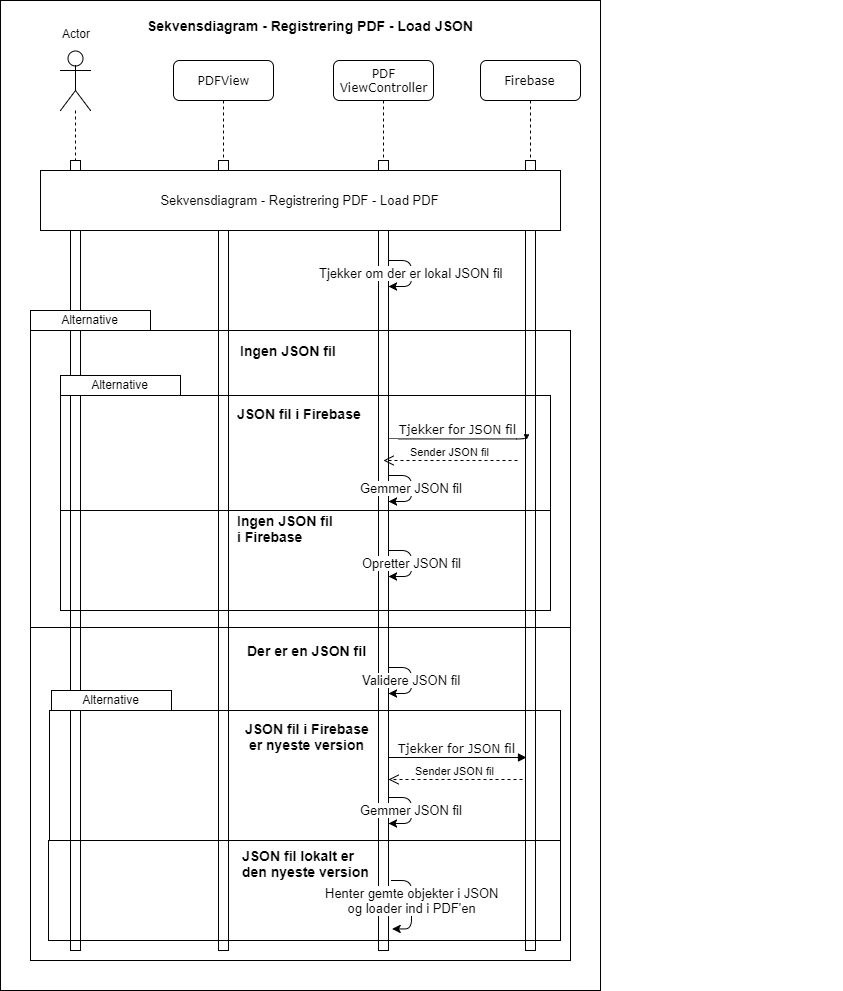
\includegraphics[height=15cm, width=15cm]{../ArkitekturDesign/Design/RegisterPDF/LoadJSONSekvensDiagram}
	\caption{Sekvensdiagram for Registrering på PDF - Loading af JSON, i Rambøll Tilsyn.}
	\label{fig:LoadJSONSekvensDiagram}
\end{figure}

\clearpage

Sidste sekvensdiagram viser, hvordan systemet opfører sig, når brugeren interagerer med applikationen i forbindelse med oprettelse af objekter på PDF-tegningen. Denne sekvens sker i forlængelse af først Loading af PDF og Load JSON. Sekvensdiagrammet for dette kan ses på Figur \ref{fig:RegistrerObjekterSekvensDiagram}.
\begin{figure}[H] % (alternativt [H])
	\centering
	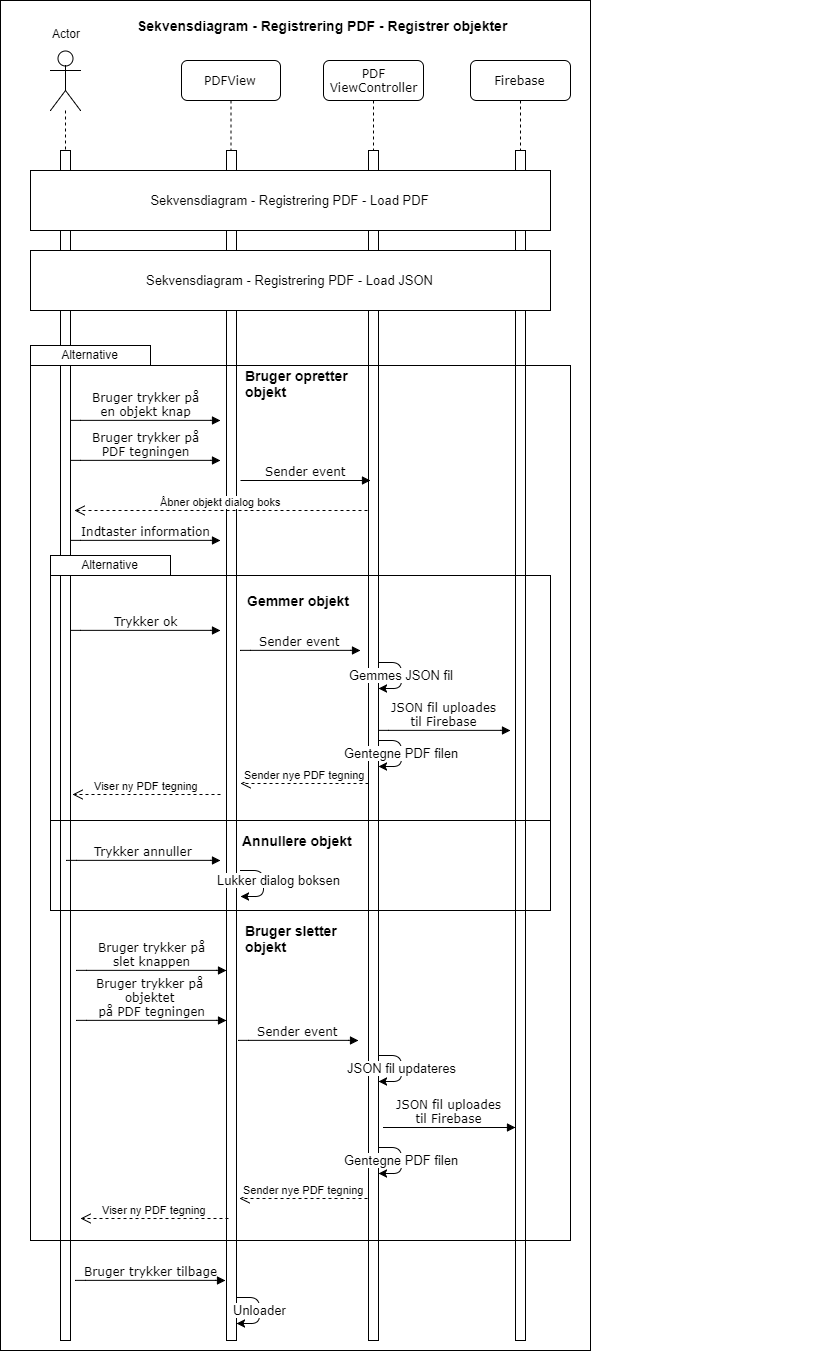
\includegraphics[height=18cm, width=15cm]{../ArkitekturDesign/Design/RegisterPDF/RegistrerObjekterSekvensDiagram}
	\caption{Sekvensdiagram for Registrering på PDF - Registrer på PDF, i Rambøll Tilsyn.}
	\label{fig:RegistrerObjekterSekvensDiagram}
\end{figure}

\clearpage

\subsubsection{Grafisk brugergrænseflade}
'Registrer på PDF' viewet, som ses på Figur \ref{fig:RegistrerObjekterView}, består af to views. Det første view viser den PDF, som er valgt til projektet. \\
Nedenunder ligger der et andet view, der indeholder knapper, som brugeren kan interagere med. Der er seks forskellige knapper: \\
Brugeren har mulighed på de første to at hoppe en side frem eller en side tilbage. \\
De næste tre knapper er symboler, som brugeren kan tegne med på PDF'en. \\
Den sidste knap er en listeknap, som giver brugeren mulighed for at afslutte sin registrering.
\begin{figure}[H] % (alternativt [H])
	\centering
	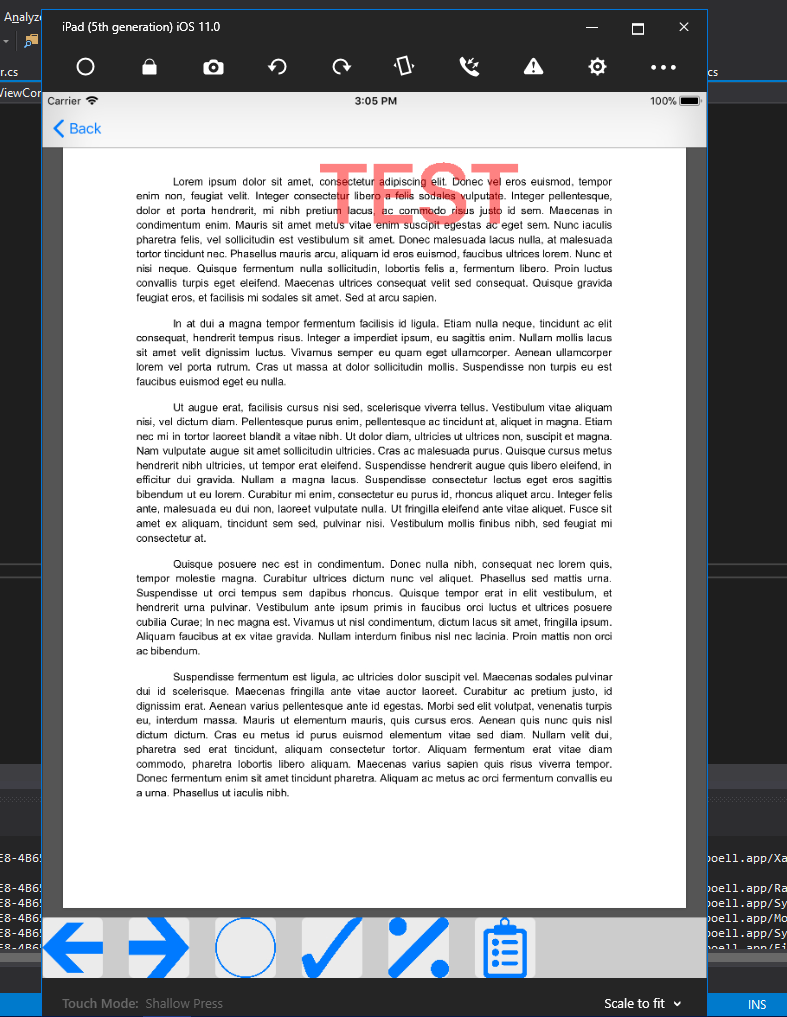
\includegraphics[height=18cm, width=15cm]{../ArkitekturDesign/Design/RegisterPDF/PDF}
	\caption{Registrer på PDF viewet, som det er implementeret i Rambøll Tilsyn.}
	\label{fig:RegistrerObjekterView}
\end{figure}

\clearpage

\subsubsection{Implementering}
I dette afsnit vil der blive beskrevet funktionaliteten for de vigtigste funktioner i koden tilhørende 'Registrering på PDF' viewet.

På Figur \ref{fig:LoadPDF} ses funktionen for LoadPDF().
\begin{figure}[H] % (alternativt [H])
	\centering
	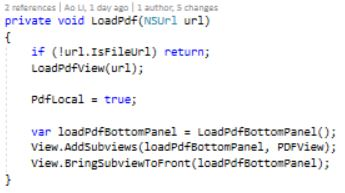
\includegraphics[height=5cm, width=10cm]{../ArkitekturDesign/Design/RegisterPDF/LoadPDF}
	\caption{Kode snip - LoadPDF() fra PdfViewController.cs}
	\label{fig:LoadPDF}
\end{figure}
Efter PDF'en er blevet downloadet fra Firebase gemmes den lokalt. \\
Det kontrolleres om url'en er en filurl. Er det en filurl loades PDF'en ind i viewet. \\
Når PDF'en er loadet ind i viewet, oprettes symbol knapperne. \\
Når både PDFViewet og PDFBottomPanel er loadet, loades disse ind i controllerens view.

\clearpage

På Figur \ref{fig:LoadPDF} ses funktionen for LoadBottomPanel().
\begin{figure}[H] % (alternativt [H])
	\centering
	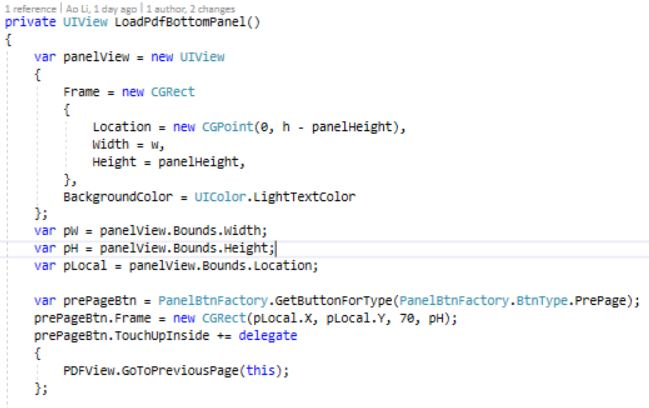
\includegraphics[height=8cm, width=15cm]{../ArkitekturDesign/Design/RegisterPDF/LoadBtnPanel1}
\end{figure}
\begin{figure}[H] % (alternativt [H])
	\centering
	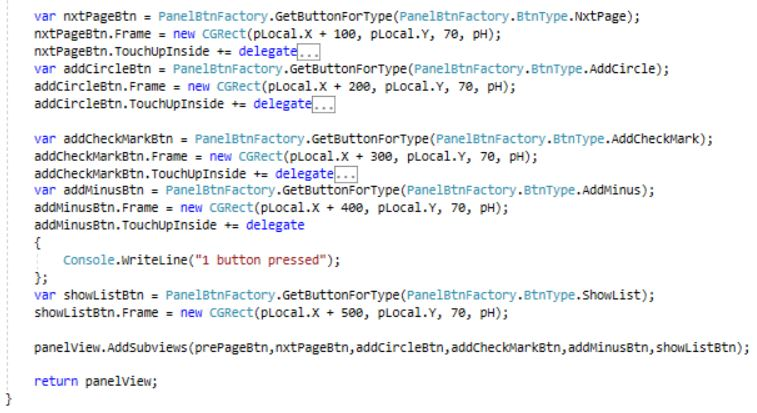
\includegraphics[height=8cm, width=15cm]{../ArkitekturDesign/Design/RegisterPDF/LoadBtnPanel2}
	\caption{Kode snip - LoadBottomPanel() fra PdfViewController.cs}
	\label{fig:LoadBtnPanel2}
\end{figure}
Her oprettes UIView, som indeholder knapper, der loades ind fra PanelBottomFactory. \\
PanelBottomFactory er en klasse, som står for at oprette knapperne. \\
Når knapperne er oprettet defineres events på de forskellige knapper. \\

\clearpage

På Figur \ref{fig:TapOnPDF2} ses funktionen for TapOnPDF().
\begin{figure}[H] % (alternativt [H])
	\centering
	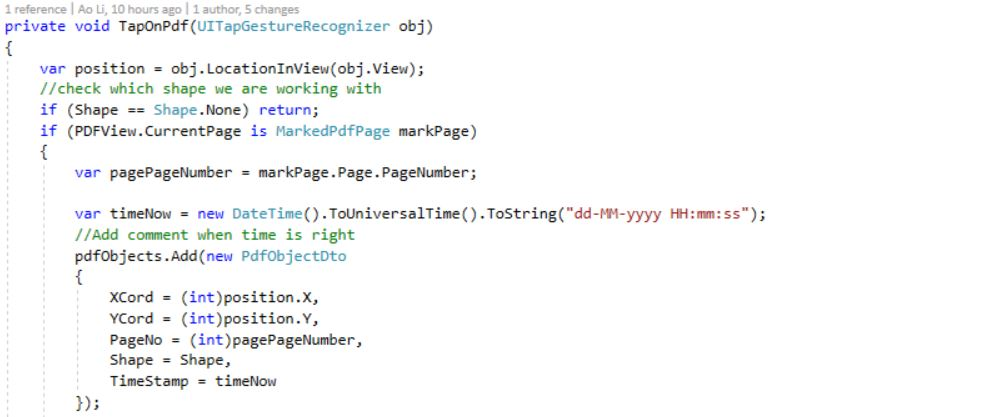
\includegraphics[height=8cm, width=15cm]{../ArkitekturDesign/Design/RegisterPDF/TapOnPDF1}
\end{figure}
\begin{figure}[H] % (alternativt [H])
	\centering
	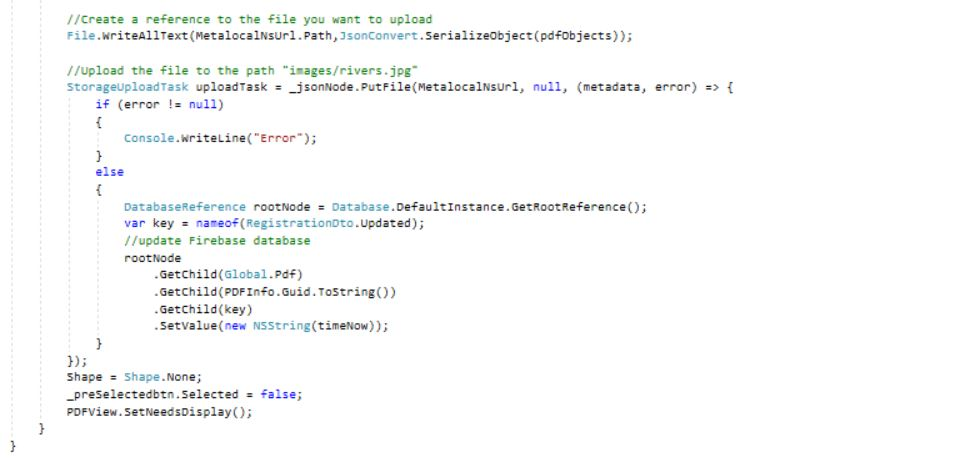
\includegraphics[height=8cm, width=15cm]{../ArkitekturDesign/Design/RegisterPDF/TapOnPDF2}
	\caption{Kode snip - TapOnPDF() fra PdfViewController.cs}
	\label{fig:TapOnPDF2}
\end{figure}


\clearpage

På Figur \ref{fig:ClassPage} ses funktionen for GetClassForPage().
\begin{figure}[H] % (alternativt [H])
	\centering
	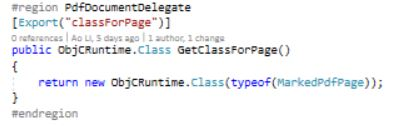
\includegraphics[height=4cm, width=10cm]{../ArkitekturDesign/Design/RegisterPDF/ClassPage}
	\caption{Kode snip - GetClassForPage() fra PdfViewController.cs}
	\label{fig:ClassPage}
\end{figure}
Funktionen ClassForPage overrides, som er en obejktive C funktion, der normalt returnerer en standard PDF page til vores typeof(MarkedPdfPage).

På Figur \ref{fig:Draw} ses funktionen for Draw().
\begin{figure}[H] % (alternativt [H])
	\centering
	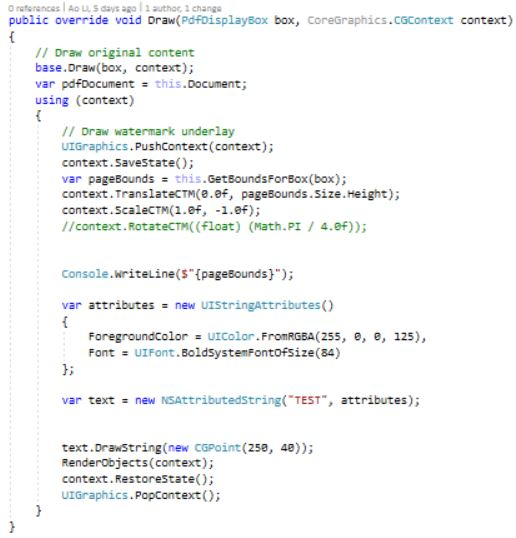
\includegraphics[height=13cm, width=15cm]{../ArkitekturDesign/Design/RegisterPDF/Draw}
	\caption{Kode snip - Draw() fra MarkedPdfPage.cs}
	\label{fig:Draw}
\end{figure}
Når PDFpagen bliver oprettet, kaldes draw, og denne er overridet til at tegne på PDF'en med de objekter, som bliver hentet fra JSON filen. Disse tegnes ind på PDF'en.

\clearpage

På Figur \ref{fig:Enum} ses Enum Shape.
\begin{figure}[H] % (alternativt [H])
	\centering
	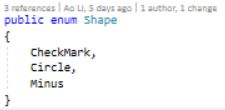
\includegraphics[height=2cm, width=5cm]{../ArkitekturDesign/Design/RegisterPDF/Enum}
	\caption{Kode snip - Enum Shape for objects fra MarkedPdfPage.cs}
	\label{fig:Enum}
\end{figure}
Definitionen på vores symboler.

På Figur \ref{fig:Singleton} ses MetaListJsonSingleton.
\begin{figure}[H] % (alternativt [H])
	\centering
	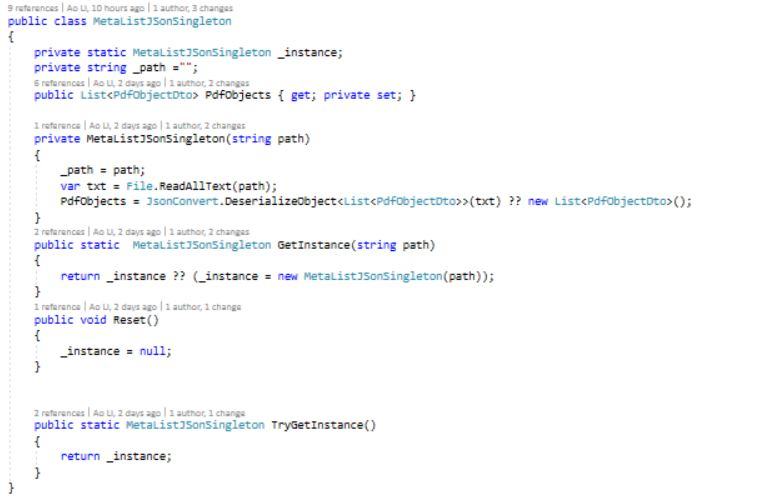
\includegraphics[height=10cm, width=14cm]{../ArkitekturDesign/Design/RegisterPDF/Singleton}
	\caption{Kode snip - MetaListJsonSingleton fra MetaListJsonSingleton.cs }
	\label{fig:Singleton}
\end{figure}
Definitionen på vores symboler.

\clearpage

På Figur \ref{fig:Render} ses funktionen for RenderObjects().
\begin{figure}[H] % (alternativt [H])
	\centering
	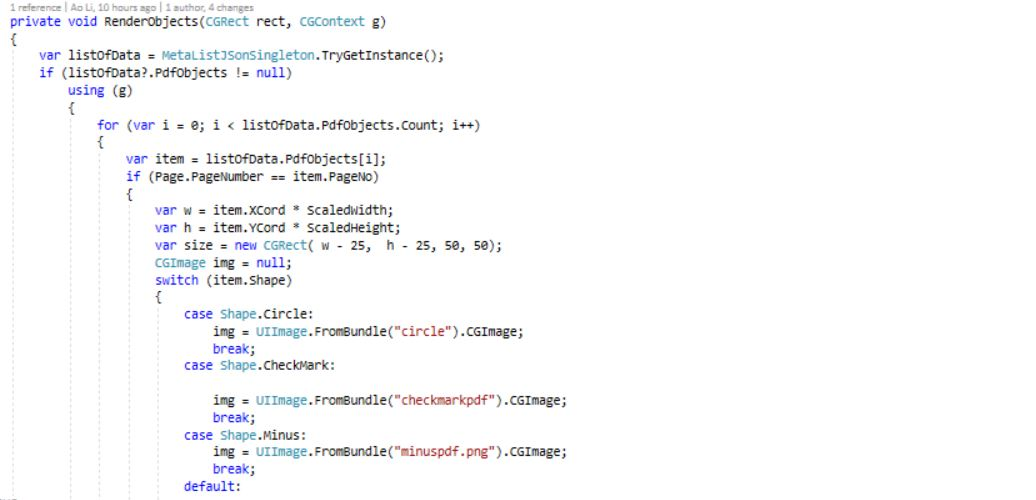
\includegraphics[height=10cm, width=15cm]{../ArkitekturDesign/Design/RegisterPDF/Render1}
\end{figure}
\begin{figure}[H] % (alternativt [H])
	\centering
	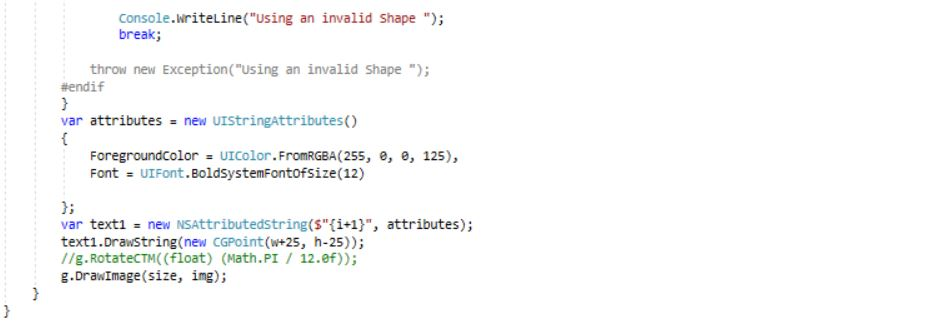
\includegraphics[height=8cm, width=15cm]{../ArkitekturDesign/Design/RegisterPDF/Render2}
	\caption{Kode snip - RenderObjects() fra MarkedPdfPage.cs}
	\label{fig:Render}
\end{figure}


\clearpage

